\section{Worst-Case Analysis}


A strictly monotonically ordered input sequence does not lead to a worst-case runtime of $O(n^2)$, as demonstrated in the previous section.
Instead, we could only show a complexity of $O(n \log n)$ for such inputs.
This use case, therefore, does not represent a true worst-case scenario for Shellsort, since the algorithm benefits from partial orderings in the $h$-sequences, as noted by \textit{Pratt}:

\blockquote[{\cite[3]{Pra72}}]{The idea underlying Shellsort is that moving elements of A long
    distances at each swap in the early stages, then shorter distances
    later, may reduce this $O(n^2)$ bound.
}\\

\noindent
To force $O(n^2)$ behavior, one must construct input sequences that provide no structural advantage during the early passes - that is , sequences that remain disordered across all $h_i$-sequences until the final pass with $h = 1$.
Recall that Shellsort in its final pass behaves like Insertion Sort, which has a worst-case runtime of $O(n^2)$ (\cite[87]{OW17b}).
Therefore, a worst-case input for Shellsort must ensure that none of the earlier $h_i$-spaced passes reduce the total number of inversions in the array.

In such a setting, the algorithm effectively performs $O(n^2)$ comparisons and swaps in the final pass alone, as all $\frac{n}{2}$ inversions must be resolved by Insertion Sort.\\

To construct such a case, we consider an array in which all elements at even indices are strictly smaller than those at odd indices.
Moreover, the elements at even and odd indices each form an increasing subsequence.
This results in a completely interleaved structure that is globally unsorted, yet locally ordered within their respective strides.
Formally, for all valid indices $i, j \in \{0, \dots, n - 1\}$ with $i < j$ and $i$ even and $j$ odd, the following conditions hold:

\[
    \begin{aligned}
        A[i] &< A[j] \\
        i + 2 &< n \;\Rightarrow\; A[i] < A[i + 2] \\
        j + 2 &< n \;\Rightarrow\; A[j] < A[j + 2]
    \end{aligned}
\]

\noindent
A sequence satisfying these constraints is illustrated in Figure~\ref{fig:worstcase_sequence}, where we are marking directly neighboured fields which exhibit an Inversion, and thus require reordering.

\begin{figure}[!h]
    \centering
    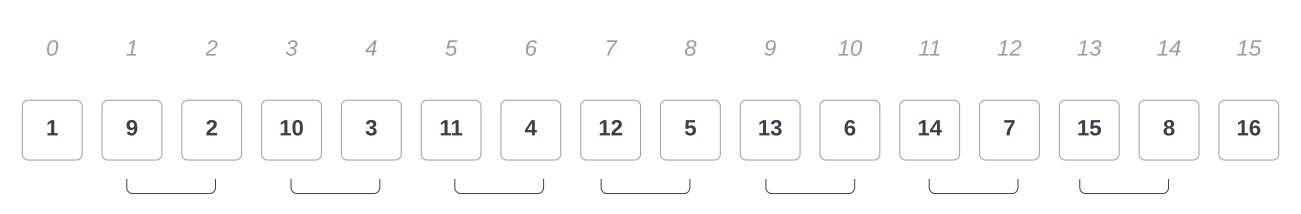
\includegraphics[width=1\columnwidth]{img/worstcase-sequence}
    \caption{A worst-case sequence for Shellsort. Fields with even index contain smaller keys than fields with odd index.}
    \label{fig:worstcase_sequence}
\end{figure}

In preceding passes with a gap of $h_s > 1$, the algorithm compares elements that are already relatively ordered and therefore does not perform any reordering.
For instance, with $h_4 = 8$, the elements $A[0..7]$ are compared with $A[8..15]$. It is easy to see that in this case
\[
    A[i] < A[j] \quad \forall\ i < j,\ j - i = 8
\]
holds, so no swaps occur.
Likewise, the next pass ($h_3 = 4$, i.e., $j - i = 4$) also does not trigger any reordering, as no inversions are found.

Only in the final pass ($h_0 = 1$), which compares adjacent elements, are inversions detected, leading to reordering (see Figure~\ref{fig:worstcase-sortsequence}).


\begin{figure}[!h]
    \centering
    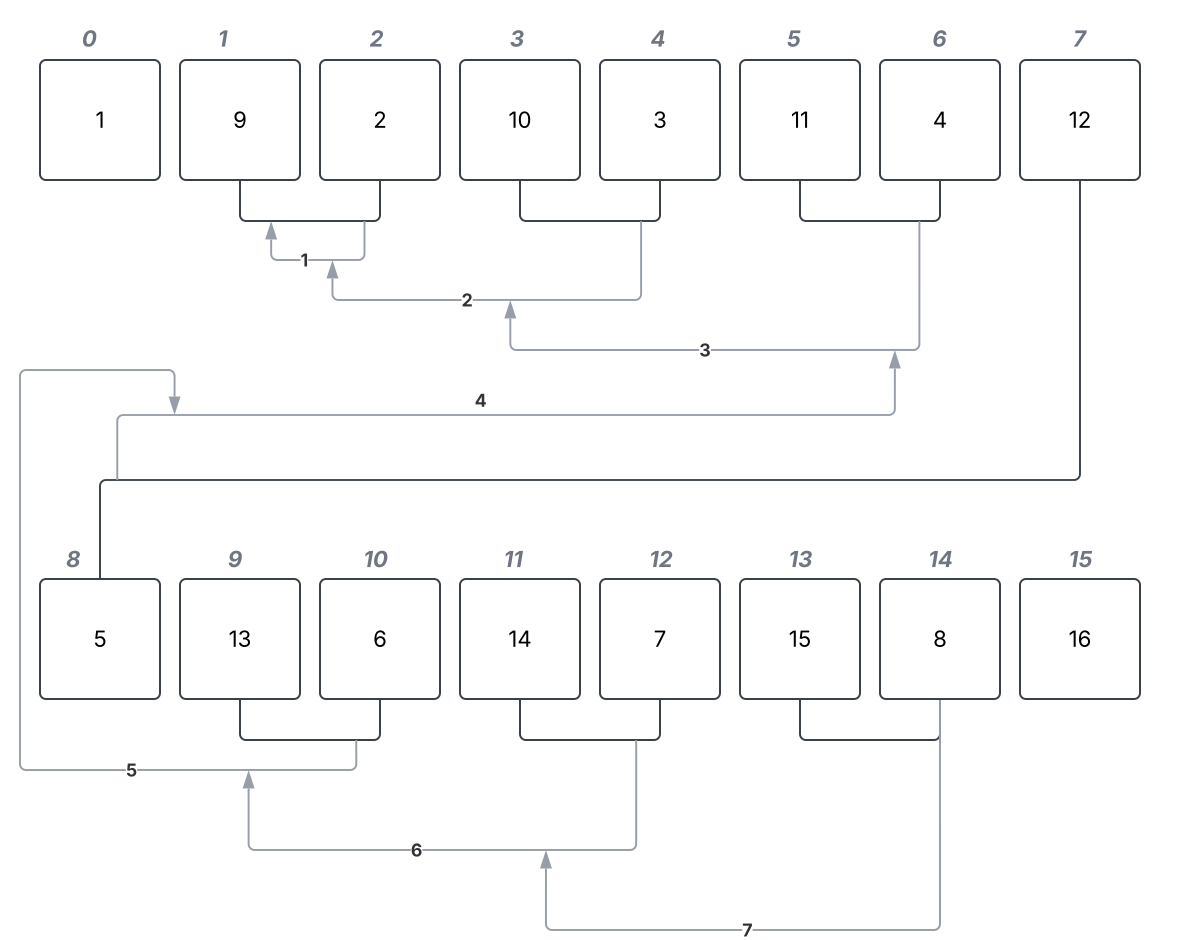
\includegraphics[width=1\columnwidth]{img/worstcase-sortsequence}
    \caption{For the worst-case sequence, the final pass detects 7 inversions. Each inversion results in a reordering by the corresponding number of positions. For $n=16$, the innermost loop $c_3$ is invoked 32 times.
}
    \label{fig:worstcase-sortsequence}
\end{figure}

\noindent
Assuming that $A[0]$ and $A[n-1]$ are already in their correct positions, the number of remaining inversions to resolve is $\frac{n}{2} - 1$.
Each inversion requires moving a key over a certain number of positions to the left.
To compute the overall cost, we sum up the necessary movements, which yields:

\[
    \sum_{i=1}^{\frac{n}{2} - 1} i = \frac{\frac{n}{2}(\frac{n}{2} - 1)}{2} = \frac{n^2 - 2n}{8}
\]

\noindent
Taking into account the previously derived contributions from $c_1$ and $c_2$, the overall step count becomes:

\[
    f(n) = \lg\ n\ + n\ \cdot \lg\ n\ - n\ + 1 +  \frac{n^2 - 2n}{8}
\]

As the quadratic term dominates for large $n$, it is easy to see that the runtime complexity is in $\boldsymbol{O(n^2)}$.